\section{Power and practical use}\label{sec:practice}

\subsection{Power}
The corrected test and the standard test apply different cutoffs to the same statistic, so their rejection regions are nested and the corrected test never has more power. The question is how much power it gives up, and how it compares with other cutoffs that are also valid. We compared four constant cutoffs on the dip, on a preregistered panel of 37 laws with 50,000 samples per law and sample size, for $n$ from 50 to 12,800.

On the null laws of the panel the uniform calibration exceeded its nominal level at every $n$, with rejection rates as high as 30.7 percent at the 5 percent level and 13.7 percent at the 1 percent level. The corrected cutoff $c_\alpha/\sqrt n$ stayed within the preregistered tolerance on every null law: the upper end of each 95 percent interval was at most $\alpha$ plus 0.5 points at the 5 percent level and $\alpha$ plus 0.25 points at the 1 percent level. Its largest rates were 4.53 and 0.90 percent, and they rose towards $\alpha$ from below as $n$ grew. Of the three cutoffs that stayed within tolerance, the corrected one is the smallest and therefore the most powerful. On the 14 alternatives whose power reached 80 percent inside the range of $n$ we simulated, half the Kuiper distance needed 1.35 to 1.55 times as many observations as $c_\alpha$, and the DKW bound 3.3 to 3.7 times. Against the uniform calibration, whose size is not controlled, the corrected test needs about twice the sample size. \Cref{fig:power} shows two symmetric normal mixtures.

\begin{figure}[t]
\centering
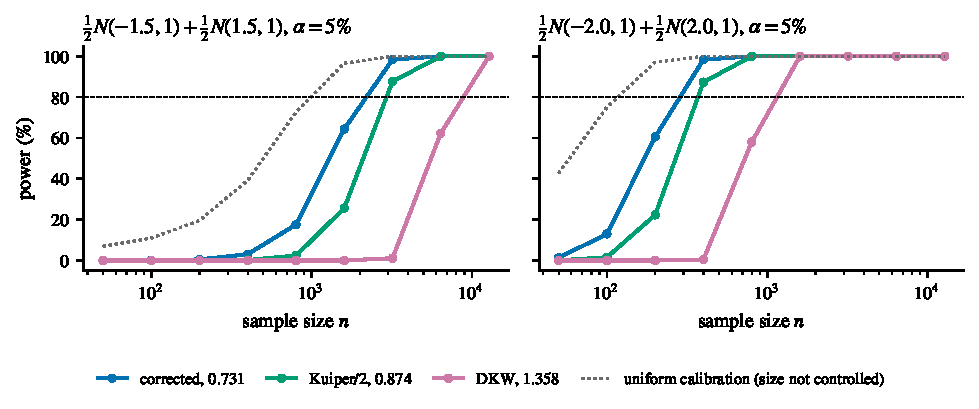
\includegraphics[width=\linewidth]{figs/fig6_power.pdf}
\caption{Among the cutoffs that keep the level, the corrected cutoff reaches high power at the smallest sample size. Power at the 5 percent level for two symmetric normal mixtures, with $50{,}000$ samples per point. Blue: the corrected cutoff $c_\alpha/\sqrt n$, asymptotically valid on $\cC$ and within tolerance on every null law of the panel. Green and purple: half the Kuiper distance and the DKW bound, valid at every $n$. Grey dotted: the uniform calibration, whose size is not controlled, shown for reference only. The dashed line marks 80 percent power.}
\label{fig:power}
\end{figure}

For small samples we compared the certified cutoffs of \cref{tab:cutoffs} with global tests of unimodality derived from the multiscale methods of Dümbgen and Walther \cite{DW08} and Rufibach and Walther \cite{RW10}. The panel had 16 bimodal laws, 11 sample sizes from 8 to 49, three levels and $10^4$ shared samples per case. The dip with certified cutoffs rejected more often in 81 to 128 of the 176 cases per comparator and level, judged by pointwise 99 percent intervals, and after a Holm correction no comparator did significantly better in any case. The multiscale methods also locate modes, which the dip does not, and we did not compare that ability. With its default grid the block criterion cannot reject at all for $n<23$.

\subsection{Data that produce flat shoulders}
The failure needs a density that is flat over a long stretch and then rises sharply. This happens when most of the data are close to uniform and a small part piles up at one end. Collections of $p$-values are the clearest example. In an exploratory screen, mixtures of uniform null $p$-values with a small fraction of strong signals near zero were rejected 11 to 22 percent of the time by the nominal 5 percent test, for $n$ between 200 and 800. The same screen found no material excess for curved pile-ups such as a censored normal, a top-coded Beta law or a zero-inflated law, so the failure does not extend to every pile-up. Among 180 published applications of the dip that we sampled, one applied it to $p$-values \cite{Roy26}.

Clustering methods inherit the calibration of the dip they call. In simulation, changing only the critical values inside the UniDip and SkinnyDip procedures \cite{Maurus16}, from the uniform table to $c_\alpha/\sqrt n$, cut the probability of splitting a unimodal feature with a flat part or a pile-up into two clusters from 13 to 29 percent down to 1 to 3 percent. The change also costs power: for one three-component mixture at $n=500$ the detection rate fell from 56 to 8.5 percent.

Two other calibrations did not solve the problem. Our implementation of the calibrated dip of Cheng and Hall \cite{CH98}, which reproduces their published table to within 1.2 points, rejected the uniform law in 30 to 81 percent of samples and $W(0.1,0.005)$ in 50 to 100 percent at the 5 percent level, for $n$ between 50 and 12,800. These laws lie outside the smoothness conditions of that method, and Cheng and Hall \cite{CH99} warned about shoulders themselves. A small neural network trained to interpolate between the uniform and the corrected cutoffs passed an internal audit, but a targeted search then found unimodal laws at which it rejected 16.9 percent of samples at the 5 percent level.

\subsection{Recommendations}
\noindent\fbox{\parbox{\dimexpr\linewidth-2\fboxsep-2\fboxrule}{\setlength{\parskip}{3pt}
\textbf{Which cutoff to use.}
\begin{itemize}[leftmargin=*,topsep=2pt]
\item $n\ge50$: reject unimodality at the 5 percent level when $\sqrt nD_n\ge0.7315$, and at the 1 percent level when $\sqrt nD_n\ge0.86$ ($0.87$ at $n=1600$). These cutoffs carry a finite-sample certificate only at the six sample sizes of \cref{tab:cutoffs}; at other $n\ge50$ they rest on the limit results, which keep the level on $\cC$ as $n\to\infty$.
\item $n=4$ and $8\le n\le49$: use the certified cutoffs of \cref{tab:cutoffs}.
\item Report a $p$-value from the uniform table only as a description of the data, not as evidence at a stated level.
\end{itemize}}}

\vspace{10pt}\noindent A user who prefers power to a size guarantee should know what the uniform table buys: false alarms on up to about a third of unimodal samples at the nominal 5 percent level.
